\section{Probase}

In our system, it is very important to understand the content of the list.
Not only is list understanding one of the goal of our project,
but also does the list content play a key role in the whole list extraction system.
Therefore we introduce Probase\cite{WuLWZ12:Probase},a probabilistic knowledge base.

Probase is a knowledge base containing a large number of real world concepts.
As is claimed in its home page\cite{ProbaseHome} that, it ``uses the world as its model'',
Probase gains knowledge from
billions of web pages and years worth of search logs.

\begin{figure}
\centering
\epsfig{file=pics/probaseOverview.eps,width=0.6\columnwidth}
\caption{A snippet of Probase's core taxonomy}
\label{fig:probaseSnippet}
\end{figure}

As is shown in Figure \ref{fig:probaseSnippet},
the knowledgebase is made up of
concepts (e.g. emerging markets and developing countries),
instances (e.g., China and India),
attributes and values (e.g., China's GDP is \$8.7 trillion),
and relationships (e.g., emerging markets, as a concept, is closely related to newly industrialized countries).
%A concept in Probase is a representation of the concept in the real world.
Just like the concept in the real world,
a concept in Probase may have instances,
attributes, relationships with other concepts.
In Probase, concepts are stored in a
taxonomic hierarchy, thus
a concept (e.g.,European Markets) can also be the instance (or subconcept) of a super concept (e.g.,Markets).

To build Probase, we need to extract concept-instance pairs,
which is pairs of ``isa'' relationships.
This is done by using syntactic patterns including the Hearst patterns\cite{Hearst92}.
For instance, for the sentence ``He is good at many instruments such as piano.'',
we can apply the the Hearst pattern ``NP such as NP'' and know that piano ``is an'' instrument.
Similarly, when extracting attributes, we can also use syntactic patterns like ``What is the NP of the NP''.
For example, assuming that we have already known that ``book'' is a concept, and ``Harry Potter'' is a instance of ``book'',
we can learn from the sentence ``Who is the author of Harry Potter?'' that ``author'' is an attribute of the concept ``book''.

\begin{table}
\centering
\caption{Scale of concept dimension\cite{ProbaseHome}}
\begin{tabular}{|l|l|l|} \hline
\textbf{name} 	& \textbf{\# of concepts}\\ \hline
Freebase 	&1,450\\
WordNet 	&25,229\\
WikiTaxonomy 	&$<$ 127,325\\
YAGO 	&149,162\\
DBPedia 	&259\\
ResearchCyc 	&$\approx$ 120,000\\
KnowItAll 	&N/A\\
TextRunner 	&N/A\\
OMCS 	&14,301\\
NELL 	&123\\
\textbf{Probase} 	&\textbf{2,653,872}\\
\hline
\end{tabular}

\label{tab:knowledgeBase}
\end{table}


Compared to other traditional knowledge bases,
Probase is distinctive in two aspects.
First, Probase is proud of a extremely large concept space. Currently it contains about 2.7 million concepts
and even more instances.
We can see from Table \ref{tab:knowledgeBase} that other existing knowledge bases have far fewer concepts,
which limit their power in modeling the real world.
Second, we say Probase is a probabilistic knowledge base, because a relation in Probase is associated with probabilities, which indicate the correctness, typicality, ambiguity, and other characteristics of the relation.
For example, instead of making an assumption that ``apple'' is an instance of ``fruit'' in other deterministic knowledge base,
we will give some values showing how likely ``apple'' is an instance of ``fruit'' in Probase.
These values are derived from evidences found in web data and other sources,
such as the frequency of the concept, instance or attribute that appears in the source.

Among the probabilistic values, two of them are of our interest:

\begin{itemize}
  \item \textit{Plausibility}:
  This value shows the certainty or confidence of a relationship.
  The higher the value is, the more certain we are that the relationship exists.
  For example, for a concept-instance pair (``fruit'',``apple''),
  the plausibility tells us how strong the fact ``apple is an instance of fruit'' is.
  With the plausibility value, we can quantifies the uncertainty,
  which is also the feature of the relationships in the real world.
  \item \textit{Typicality}:
  In terms of probability theory, it is defined as the conditional probability
  of a concept/instance given an instance/concept.
  Generally we use $P(C|I)$ or $P(C|I)$ to represent the typicality.
  Intuitively, the typicality measures how strong the relation between a concept and an instance is.
  For example, $P(C=company|I=apple)$ shows how likely people think of the concept ``company'' when they see the word ``apple'';
  while $P(I=steve jobs|C=ceo)$ indicates how likely ``steve jobs'' will come into mind when people think about the concept ``ceo''.
  We can use the following euqations to estimate typicality:
  \begin{eqnarray}
  \label{equ:typicality}
    P(I|C) = \frac{N(C, I)}{N(C)+\alpha} \\
    P(C|I) = \frac{N(C, I)}{N(I)+\alpha}
  \end{eqnarray}
    where $N(x)$ is the frequency of the occurrence of concept/instance $x$,
    $N(x,y)$ is the frequency of the occurrence of the concept-instance pair $(x,y)$.
    In these equations, factor $\alpha$ is introduced for Laplace smoothing\cite{lidstone1920note}.
\end{itemize}

There are a lot of applications of Probase,
among which short text conceptualization is of our interest, and we will discuss it in Section \ref{sec:shortText}.


%
%The distinctive aspect of Probase compared with other knowledge
%bases is that, in Probase, the relation between a concept and
%subconcept or a concept and an instance is not defined in a strict
%well-defined manner. Each relation is given a probability value
%which measure the \textit{value} of the relationship. The first
%value called \textit{plausibility} value, measures how strong or
%certain we are that a concept and a subconcept is actually related.
%Take an example of pair (``animals'',``reptiles''). The plausibility
%value tells us how strong that the 'reptiles' is seen as 'animals' or
%how certain we are that 'reptiles' is indeed 'animals'. This degree
%of uncertainty is important since it represents how exactly the
%concepts in the real world is attached to each other.
%
%Another value that is a subject of interest to us in this work is
%the \textit{typicality} value. It measures how strong the relation
%between a concept and an instance. We take use of this value as one
%of the components to measure the relevancy between the concepts in
%user query and the instances found in queries from query log. The
%value is derived as:
%
%\[Typicality\textnormal{-}value(i, c) = \frac{n(i, c)}{n(c)+\alpha}\]
%
%where $i$ is an instance and $c$ is a concept. The $n(i,c)$ is the
%frequency of the occurrence of instance $i$ and concept $c$ together
%in extracted pairs from web pages, and $n(c)$ is the frequency of the
%occurrence of concept $c$ in all pairs. The value $\alpha$ is used
%to smooth the score and to avoid the high typicality value of a
%concept $c$ that only have one instance $i$, which can be harmful
%if the relationship is supposed to be small. To show how typicality
%value can be used, take an example of an instance ``boa''. The
%typicality value of pair (``boa'',``snakes'') is 0.0138 while the pair
%(``boa'',``korean singers'') has typicality value of 0.00197. From
%this result, we can see that ``boa'' is more likely known as a name
%of a snake than as the name of a singer.

%Another feature of Probase is that it is probabilistic, which means every claim in Probase is associated with some probabilities that model the claim��s correctness, typicality, ambiguity, and other characteristics. The probabilities are derived from evidences found in web data, search log data, and other existing taxonomies. For example, for typicality (between concepts and instances), Probase contains the following probabilities:
%
%    P(C=company|I=apple): How likely people will think of the concept ��company�� when they see the word ��apple��.
%    P(I=steve jobs|C=ceo): How likely ��steve jobs�� will come into mind when people think about the concept ��ceo��.
%
%Probase also has typicality scores for concepts and attributes. Another important score in Probase is the similarity between any
%two concepts y1 and y2 (e.g., celebrity and famous politicians). Thus Probase can tell that natural disasters and politicians are very different concepts, endangered species and tropical rainforest plants have certain relationships, while countries and nations are almost the same concepts.
%
%These probabilities serve as priors and likelihoods for Bayesian reasoning on top of Probase. In addition, the probabilistic nature of Probase also enables it to incorporate data of varied quality from heterogeneous sources. Probase regards external data as evthese probabilities serve as priors and likelihoods for Bayesian reasoning on top of Probase.
%
%Probase is a probabilistic knowledge base, built by
%extracting pairs of \textit{isA} relationship of concepts
%from web pages. In Probase, concepts are stored in a
%taxonomic manner. Currently, it contains around 2.7
%million concepts that were extracted from more than 1
%billion web pages. A concept in Probase can be seen as
%a representation of object in real world. An instance
%can also be considered as a single concept, which cannot
%be instantiated into other concepts or instances. Figure
%\ref{fig:exampleProbase} shows the example for this relation.
%
%
%
%
%
%We can see from this figure, that ``animals'', ``livestocks'',
%``reptiles'', ``snakes'', ``korean singers'' are regarded as
%concepts, and ``boa'' as an instance. A concept may be a
%subconcept of other concept, e.g. ``snakes'' is a subconcept
%of ``animals''.
%
%
%
%The distinctive aspect of Probase compared with other knowledge
%bases is that, in Probase, the relation between a concept and
%subconcept or a concept and an instance is not defined in a strict
%well-defined manner. Each relation is given a probability value
%which measure the \textit{value} of the relationship. The first
%value called \textit{plausibility} value, measures how strong or
%certain we are that a concept and a subconcept is actually related.
%Take an example of pair (``animals'',``reptiles''). The plausibility
%value tells us how strong that the 'reptiles' is seen as 'animals' or
%how certain we are that 'reptiles' is indeed 'animals'. This degree
%of uncertainty is important since it represents how exactly the
%concepts in the real world is attached to each other.
%
%Another value that is a subject of interest to us in this work is
%the \textit{typicality} value. It measures how strong the relation
%between a concept and an instance. We take use of this value as one
%of the components to measure the relevancy between the concepts in
%user query and the instances found in queries from query log. The
%value is derived as:
%
%\[Typicality\textnormal{-}value(i, c) = \frac{n(i, c)}{n(c)+\alpha}\]
%
%where $i$ is an instance and $c$ is a concept. The $n(i,c)$ is the
%frequency of the occurrence of instance $i$ and concept $c$ together
%in extracted pairs from web pages, and $n(c)$ is the frequency of the
%occurrence of concept $c$ in all pairs. The value $\alpha$ is used
%to smooth the score and to avoid the high typicality value of a
%concept $c$ that only have one instance $i$, which can be harmful
%if the relationship is supposed to be small. To show how typicality
%value can be used, take an example of an instance ``boa''. The
%typicality value of pair (``boa'',``snakes'') is 0.0138 while the pair
%(``boa'',``korean singers'') has typicality value of 0.00197. From
%this result, we can see that ``boa'' is more likely known as a name
%of a snake than as the name of a singer.

\section{Short Text Conceptualization}
\label{sec:shortText}

Short text conceptualization is an interesting NLP problem.
Basically, given a list of words as short text,
the task is to assign a concept that can best match the topic of the short text.
For example, given a word list \{``India'',``China''\}, we may conceptualize it as ``Asian countries'';
then if we expand the list to \{``India'',``China'',``Brazil''\}, the best match becomes ``BRIC countries''.
In our project, we want to conceptualize extracted lists, which is very similar to short text (and even more similar to word lists).
Therefore, we may apply the technologies of this field in our system.

This problem is especially challenging because short texts lack
enough content from which statistical conclusions
can be drawn easily.
In addition, a short text like a tweeter may not follow close to the line of linguistic grammar,
which make it difficult to get correct parsing result from normal NLP tools like Stanford Parser.
Among many effort to this task\cite{gabrilovich2005feature,egozi2008concept}, the work of Yangqiu et al. \cite{Song11:Conceptualize} is impressive.
In their paper, they propose a method of conceptualizing short text using Probase as knowledgebase, in which
probabilistic framework  is built using Naive Bayesian Model.
To evaluate their method, they conduct a series of experiments with thousands of tweets data,
the result shows that their system outperforms all other existing approaches.

The algorithm for conceptualization consists of three parts: instance conceptualization, attribute conceptualization and mixed models.
These methods are similar in mechanism, and for our project we are only interested in instance lists.
Therefore we will focus on instance conceptualization in the following.

Given a set of observed instances $E=\{e_{i},i \in 1,...,M\}$, our goal is to generate a set of most representative
concepts that can best describe the instance set $E$. The probability of concepts can be estimated by a Naive Bayesian Model.

\begin{equation}\label{equ:shortText1}
    P(c_{k}|E)=\frac{P(E|c_{k})P(c_{k})}{P(E)}
    \propto P(c_{k})\prod_{i=1}^{M}P(e_{i}|c_{k}).
\end{equation}

In Equation \ref{equ:shortText1}, $P(e_{i}|c_{k})$ is the typicality of the instance $e_{i}$ given the concept $c_{k}$,
which can be calculated by Equation \ref{equ:typicality}; $P(c_{k})$ is approximately proportional
to the observed frequency $N(c_{k})$.
Apparently, the concept $c_{k}$ with the max posterior probability is considered as the best matched concept.





